\documentclass[a4paper,UTF8]{article}
\usepackage{ctex}
\usepackage[margin=1.25in]{geometry}
\usepackage{color}
\usepackage{graphicx}
\usepackage{amssymb}
\usepackage{amsmath}
\usepackage{amsthm}
\usepackage{booktabs}
\usepackage{caption}
\usepackage{fancyhdr}
\usepackage{extramarks}
\usepackage{amsfonts}
\usepackage{tikz}
\usetikzlibrary{arrows}
\usepackage{algorithm}
\usepackage{algorithmicx}
\usepackage{algpseudocode}
\usepackage{listings}

%\usepackage[thmmarks, amsmath, thref]{ntheorem}
\theoremstyle{definition}
\newtheorem*{solution}{Solution}
\newtheorem*{prove}{Proof}
\usepackage{multirow}

%
% Basic Document Settings
%

\topmargin=-0.45in
\evensidemargin=0in
\oddsidemargin=0in
\textwidth=6.5in
\textheight=9.0in
\headsep=0.25in

\linespread{1.1}

\pagestyle{fancy}
\lhead{\hmwkTitle}
\chead{\hmwkClass\ (\hmwkClassInstructor\ \hmwkClassTime)}
\rhead{\hmwkAuthorName}
\lfoot{\lastxmark}
\cfoot{\thepage}

\renewcommand\headrulewidth{0.4pt}
\renewcommand\footrulewidth{0.4pt}

%
% Homework Details
%   - Title
%   - Due date
%   - Class
%   - Section/Time
%   - Instructor
%   - Author
%

\newcommand{\hmwkTitle}{Assignment \ \#5}
\newcommand{\hmwkDueDate}{Oct 6, 2017}
\newcommand{\hmwkClass}{Problem Solving}
\newcommand{\hmwkClassTime}{}
\newcommand{\hmwkClassInstructor}{Professor Chen}
\newcommand{\hmwkAuthorName}{李志琦 161220074}

%--

%--
\begin{document}


\subsection*{26.1-1}
because id x = od x = 1  for G', any flow  going through  u-x, it will go though x-v.

any flow going through x-v,it comes from u-x. so u-x and x-v always have same flow,

we can see them as a flow u-v. so G and G' can be seen as  same graph and has same flow.

\subsection*{26.1-2}
if the graph has n sources.

the flow of multiple-source, multuple-sink problem is $|\sum_{i=1}^{n} \sum_{v \in V}f(s_i,v)-\sum_{v \in V}f(v,s_i)|$

if add a supersource and a supersink, the flow is $| \sum_{v \in V'}f(s_s,v)- \sum_{v \in V'}f(v,s_s)|$ because there aren't flow from vertex to $s_s$
so the flow is $| \sum_{v \in V'}f(s_s,v)|$ , and if there is a flow from $s_s$ to v, v is $s_i$,
so the flow is $| \sum_{i=1}^{n}f(s_s,s_i)|$, for all $s_i$, because flow conservation so the flow in $s_i$ is equal to the flow out from $s_i$
so $| \sum_{i=1}^{n}f(s_s,s_i)|$=$|\sum_{i=1}^{n} \sum_{v \in V}f(s_i,v)-\sum_{v \in V}f(v,s_i)|$.
\subsection*{26.1-6}
let home be source s, and school be sink t, and each road be a edge with capacity 1, and each corner be a vertex.
so if the maxflow if not less than 2, his children can go to school safely. because every edge's capacity is 1, each unit flow gose throgh the edges that no other
flow gose through.
\subsection*{26.1-7}
split each vetex v in G into 2 vertices $v_1,v_2$ in $G'$ and add a edge between these two vertices, and its capacity is l(v)
and if there is an edge (u,v) in G ,then add an edge between $u_1,v_0$ with the capacity of c(u,v) in G
so the number of edge is $|V|$ and the number of vertex is $|V|+|E|$

\subsection*{26.2-2}
the flow is 11+1-4+7+4 = 19

the capacity is 16 + 4 + 7 + 4 = 31
\subsection*{26.2-4}
A minimum cut  is S = {s, v1, v2, v4} and T = {v3, t}.

The augmenting path in part (c) cancels flow on edge (v3, v2).

\subsection*{26.2-6}
add a supersource s and a supersink t . and then add a vertex $s_i'$ between each $s_i$ and s. remove $s_i$-$s$

and let the capacity of  $s_i$-$s_i'$ is $p_i$ and the capacity of $s_i'$-$s$ be $\infty$

and add a vertex $t_i'$ between each $t_i$ and t, remove $t_i$-$t$

and let the capacity of  $t_i$-$t_i'$ is $q_i$ and the capacity of $t_i'$-$t$ be $\infty$
\subsection*{26.2-8}
if we use bfs algorithm to find augmenting path, no edge in s will appear in it.
so it doesn't matter having edges into s.
\subsection*{26.2-10}
first we find the maximum flow use ordinary way. then we create a new graph G',and the vertices set and edge set are same as G,
and each edge u-v's capacity is the maximum flow f(u,v). so each time we find a augmenting path, we will remove the edge whose
flow equals to its capacity, so this edge won't appear in residual network. once we find a augmenting path ,the number of edge decrease at least one.
so there are at most |E| augmenting path. it is correct, bacause we actually do not need cancel flow and the capacity in G' is maxmum flow in G.

\subsection*{26.2-12}
because the f(v,s)'s  flow actually comes from s, obviously  there is a circle from s to s, and the flow on it is f(v,s), so we just
remove the flow on the circle and it won't influence the maximum flow. so there must exist another flow f=0 with $f'(v,s)=0$; such that
|f|=|f'|.

use dfs to find such a circle and decrease the flow of each edge on the circle to 0. it is O(|E).
\subsection*{26.2-13}

\subsection*{26.3-3}

first we observe the graph follwing, if we want to find a longest path start at left vertices and end at right vertices and each edge incident with both left and right

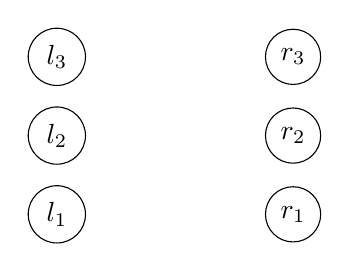
\begin{tikzpicture}
\tikzset{vertex/.style = {shape=circle,draw,minimum size=0.5em}}
\tikzset{edge/.style = {->,> = latex'}}
% vertices
\node[vertex] (s) at  (0,0) {$l_1$};
\node[vertex] (u) at  (0,1) {$l_2$};
\node[vertex] (v) at  (0,2) {$l_3$};
\node[vertex] (s) at  (3,0) {$r_1$};
\node[vertex] (u) at  (3,1) {$r_2$};
\node[vertex] (v) at  (3,2) {$r_3$};
%edges
%\draw[edge] (s) to   (u);
%\draw[edge] (u) to   (v);
%\draw[edge] (v) to   (s);
\end{tikzpicture}

the path is like this, and it's length is 2*3-1

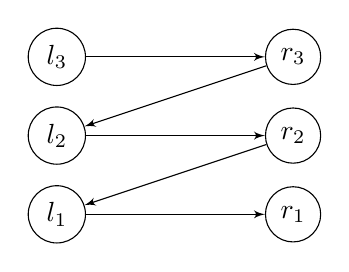
\begin{tikzpicture}
\tikzset{vertex/.style = {shape=circle,draw,minimum size=0.5em}}
\tikzset{edge/.style = {->,> = latex'}}
% vertices
\node[vertex] (l1) at  (0,0) {$l_1$};
\node[vertex] (l2) at  (0,1) {$l_2$};
\node[vertex] (l3) at  (0,2) {$l_3$};
\node[vertex] (r1) at  (3,0) {$r_1$};
\node[vertex] (r2) at  (3,1) {$r_2$};
\node[vertex] (r3) at  (3,2) {$r_3$};
%edges
\draw[edge] (l3) to   (r3);
\draw[edge] (r3) to   (l2);
\draw[edge] (l2) to   (r2);
\draw[edge] (r2) to   (l1);
\draw[edge] (l1) to   (r1);
\end{tikzpicture}

so then we want to construct a graph like following and it's longest augmenting path in 2*min(|L|,|R|)+1
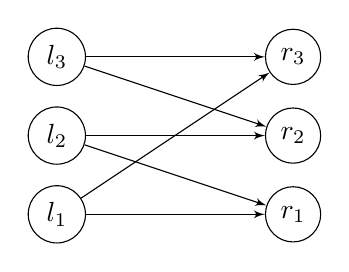
\begin{tikzpicture}
\tikzset{vertex/.style = {shape=circle,draw,minimum size=0.5em}}
\tikzset{edge/.style = {->,> = latex'}}
% vertices
\node[vertex] (l1) at  (0,0) {$l_1$};
\node[vertex] (l2) at  (0,1) {$l_2$};
\node[vertex] (l3) at  (0,2) {$l_3$};
\node[vertex] (r1) at  (3,0) {$r_1$};
\node[vertex] (r2) at  (3,1) {$r_2$};
\node[vertex] (r3) at  (3,2) {$r_3$};
%edges
\draw[edge] (l3) to   (r3);
\draw[edge] (l3) to   (r2);
\draw[edge] (l2) to   (r2);
\draw[edge] (l2) to   (r1);
\draw[edge] (l1) to   (r1);
\draw[edge] (l1) to   (r3);
\end{tikzpicture}

first we find 2 augmenging path $l_1-r_1$,$l_2-r_2$,after that we can find a longest  augmenting path
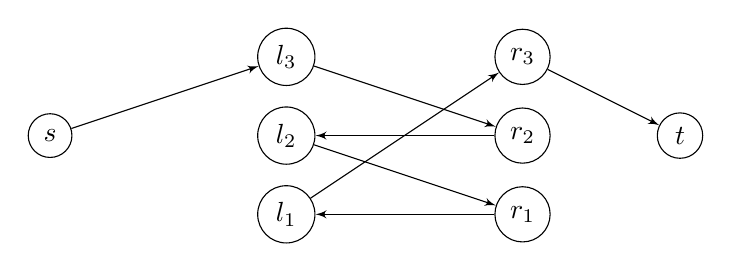
\begin{tikzpicture}
\tikzset{vertex/.style = {shape=circle,draw,minimum size=0.5em}}
\tikzset{edge/.style = {->,> = latex'}}
% vertices
\node[vertex] (s) at  (0,1) {$s$};
\node[vertex] (l1) at  (3,0) {$l_1$};
\node[vertex] (l2) at  (3,1) {$l_2$};
\node[vertex] (l3) at  (3,2) {$l_3$};
\node[vertex] (r1) at  (6,0) {$r_1$};
\node[vertex] (r2) at  (6,1) {$r_2$};
\node[vertex] (r3) at  (6,2) {$r_3$};
\node[vertex] (t)  at  (8,1) {$t$};
%edges
\draw[edge] (s) to   (l3);
\draw[edge] (l3) to   (r2);
\draw[edge] (r2) to   (l2);
\draw[edge] (l2) to   (r1);
\draw[edge] (r1) to   (l1);
\draw[edge] (l1) to   (r3);
\draw[edge] (r3) to   (t);
\end{tikzpicture}

as for the general graph, if |L|!=|R| we choose m=min(|L|,|R|) and the longest path is
2m+1. so the upperbound is 2min(|L|,|R|) + 1

\subsection*{26.1}
\subsubsection*{a}
see 26.1-7
\subsubsection*{b}
first we consrtuct a vertex constrained flow network G. and each intersection is a vertex in
G with capacity 1, and each line between two vertices in grid will be a bidirectional edge in G woth capacity 1.
and then we add a supersource  s and add a edge with capacity 1 between s and the vertex which is start  point in grid.
and add a supersink t and add a edge with capacity 1 between t and the vertex which lies on the boundary.
so we can transform this graph into a edge constrained flow network. and use a maxium flow algorithm.
if the flow is m, can escape. the final graph has V=$2n^2+2$ vertices and $E^2=n^2+2n(n-1)+m+(4n-4)$ edges
time by using  maximum flow algorithm is $O(VE^2)$ and other running time is $O(V+E)$
so the totally running time is $O(VE^2)$ V=$2n^2+2$  and $E^2=n^2+2n(n-1)+m+(4n-4)$

\subsection*{26.2}
\subsubsection*{a}

use the graph G'. and let the capacity of each edge be 1. and then run the maxmimum flow algorithm.
suppose the result is f, and the the fewest paths is n-k.

because we know the G' is a Maximum bipartite matching. and every edge $x_i-y_j$ in G' equals to (i,j) is an edge in path cover.
one edge$(x_i-y_i)$ in G' equals one unit flow, equals one edge in path cover. so there are f edges cover n vertices so there are n-f paths.

\subsubsection*{b}
no,  in Maximum bipartite matching ,if there is an edge $x_i-y_j$ in G', there won't be  $x_i-y_m$(m!=j) and  $x_n-y_j$ (n!=i) in maximum flow.
but if the graph has a circle, we maybe need that a vertex incident from  more than one vertex of incident to more than one vertex like the vertex b in following incident from more than one vertex .

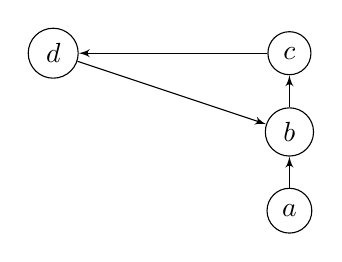
\begin{tikzpicture}
\tikzset{vertex/.style = {shape=circle,draw,minimum size=0.5em}}
\tikzset{edge/.style = {->,> = latex'}}
% vertices

\node[vertex] (a) at  (3,0) {$a$};
\node[vertex] (b) at  (3,1) {$b$};
\node[vertex] (c) at  (3,2) {$c$};
\node[vertex] (d) at  (0,2) {$d$};

%edges
\draw[edge] (a) to   (b);
\draw[edge] (b) to   (c);
\draw[edge] (c) to   (d);
\draw[edge] (d) to   (b);

\end{tikzpicture}
\end{document}
